\section{Current State of ECDAR}
This section describes the current state of the ECDAR GUI and the Reveaal engine, followed by an exploration of the future plan for ECDAR.

\subsection{State of GUI} 
The GUI is split into three vertical panes, as seen in \autoref{fig:ECDAR-gui}. The different components in the project are listed in the project pane to the left, the currently selected component is shown in the editor pane in the middle, and the queries are found in the query pane to the right. Through the editor pane, components can be created, modified and deleted. Projects are saved in their own folders with a JSON file for each component, allowing the components to be used for queries in the engines of ECDAR.
The GUI also has a top bar, from where it is possible to open a project, hide panes, choose engine options, and more.  
Additionally, the GUI has a bar at the bottom of the view. Here, errors and warnings are supposed to be displayed.

\begin{figure}[H]
    \centering
    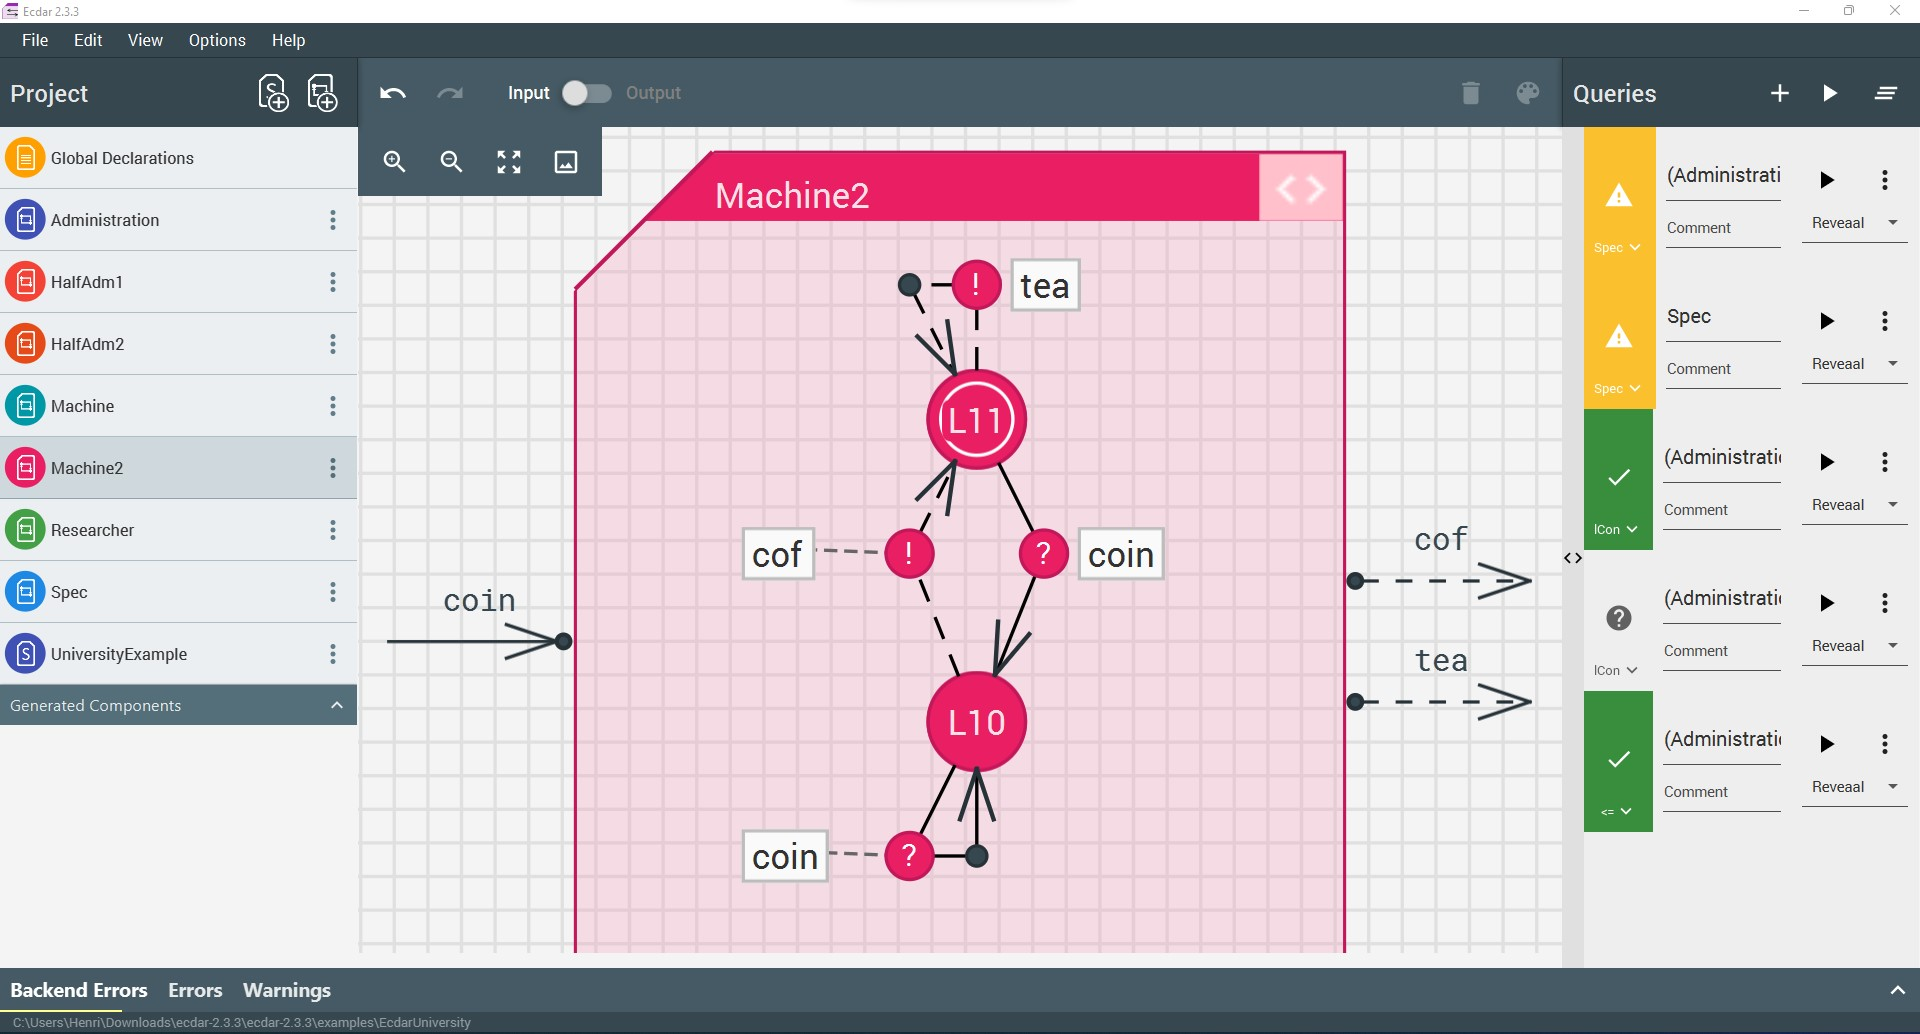
\includegraphics[width=1\textwidth]{common/figures/ecdar-overview.jpg}
    \caption{A screenshot of the ECDAR GUI of the latest version (ECDAR 2.3.3 released on 2022-09-08) \cite{ECDARNETreleasenotes}.}
    \label{fig:ECDAR-gui}
\end{figure}

In the example above, \textit{Machine2} is selected and viewed in the editor pane. \textit{Machine2} is a model of a coffee machine. The accepted input is shown on the left side of the component as a solid arrow pointing towards the component, here the input is \texttt{coin}. On the right side the output from the coffee machine, namely \texttt{cof} and \texttt{tea}, is illustrated with dashed arrows pointing away from the component. 
Inside the component, the model is composed of locations in the shape of big circles, and transitions marked by arrows between the locations. The initial location, \texttt{L11}, is marked by a white circle around the text.
The two different types of transitions (input and output) are distinguishable through the type of line (solid or dashed), and through the symbols in the small circles on the arrows. The exclamation mark indicates an output, e.g., tea on the transition from location \texttt{L11} to itself at the top of the model. A question mark, on the other hand, indicates an input. An example of that is the transition from \texttt{L11} to \texttt{L10}.

Apart from the mentioned features, it is also possible to add guards and updates, in addition to invariants by right-clicking the transitions and locations, respectively. An example of a guard is provided in \autoref{fig:ECDAR-guard} as a circle containing the less-than symbol with an associated text box in which the actual guard is added and can be edited. 
An update is represented in a similar manner, but with the equals symbol in the small circle. This is shown in \autoref{fig:ECDAR-guard} on the transition from \texttt{L5} to \texttt{L4}.

\begin{figure}[H]
    \centering
    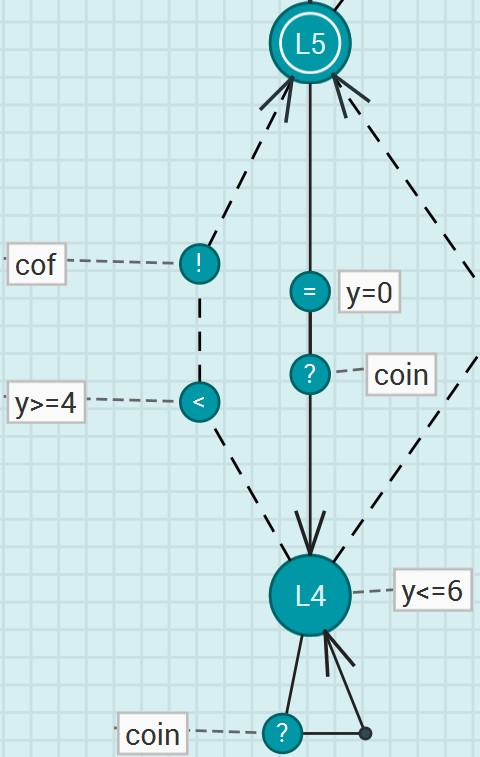
\includegraphics[width=0.3\textwidth]{common/figures/ecdar-guards.jpg}
    \caption{A screenshot of a model containing guards, updates, and invariants.}
    \label{fig:ECDAR-guard}
\end{figure}

An example of an invariant can be seen in \autoref{fig:ECDAR-guard} as a text box with a dashed line connecting it to location \texttt{L4}. The invariant is edited in a manner similar to that of the guards and updates. 

As mentioned earlier, queries can be executed from the query pane to the right of the GUI, removing the necessity of using the CLI for query execution. Here all created queries can be run at once or individually. A query consists of a query request specified in the text-field, a query type chosen using the drop-down underneath the icon, and the selection of a backend engine for execution. The drop-down menu contains a preset of query types, but not all options are currently supported with functionality that being e.g. reachability. 

The run of a query can result in one of three things: A green box that indicates a successful run, a yellow box that indicates the query could not be parsed by the GUI or other issues occurring on the GUI, or a red box that indicates that the query is unsuccessful e.g. some check in engine fails.

\begin{figure}[H]
    \centering
    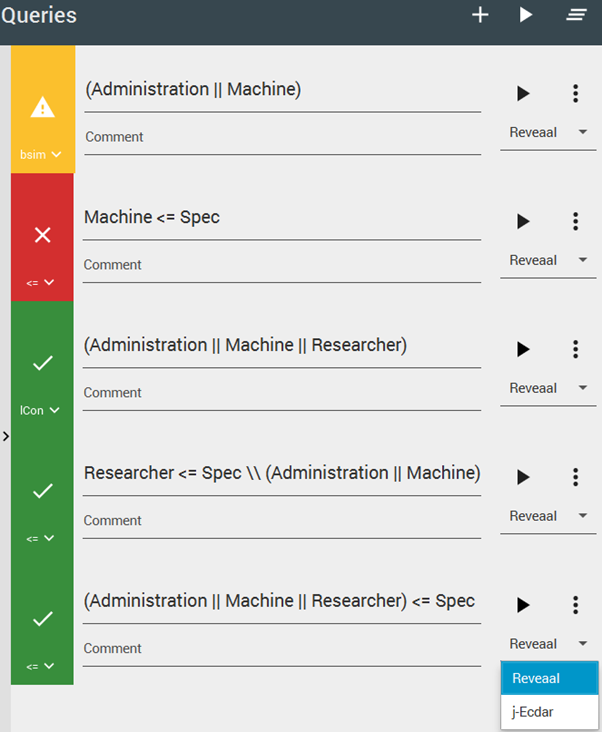
\includegraphics[width=0.6\textwidth]{common/figures/right-panel.png}
    \caption{A screenshot of the query pane.}
    \label{fig:ECDAR-queries-panel}
\end{figure}

\autoref{fig:ECDAR-queries-panel} shows five different queries. 
The result of the first query in the query pane is an error, which means the GUI could not handle the query. 
Underneath this query, the "Machine$<=$Spec" query is performed. The result of this query is unsuccessful.
The three remaining queries are all successful and without errors.
Further information about the results of the queries can be read by hovering the mouse over the colored icons.


\subsection{State of Reveaal}
Reveaal is a system designed to check the correctness of a real-time Compositional System, made by a model designer. It is able to test a variety of different types of queries, such as refinement and consistency, making it a powerful tool for ensuring the correctness of the systems. Reveaal uses a gRPC framework implementation, allowing for quick and easy communication between model designers choice of frontend and the engine itself. ECDAR does, however, currently only has a single GUI. The Executable Query handler within Reveaal is responsible for recognizing the type of query it receives, and then call the correct functions to perform the query. Upon completion of the query, Reveaal will return either a success or an error, again using gRPC. All in all, Reveaal is a powerful engine for ensuring the accuracy of Compositional Systems.

Though Reveaal provides basic functionalities outlined in the theory paper, its error handling and user-friendliness leave much to be desired. Errors are not communicated to a user as the Reveaal engine just panics, leading to a generic error message in the GUI, which does not provide any information regarding the violating action or the unreachable part of the model. Consequently, users are not provided with an optimal experience. Further work is necessary to ensure that Reveaal is able to deliver the user-friendly experience required to reach its full potential.

\subsection{Plan for ECDAR} \label{sec:plan-for-ecdar}
During the project period, the state of ECDAR should evolve to encompass more features, and by those means, be more complete. Each team is assigned a part of ECDAR to work on, there are five teams working on the Reveaal Engine, and one team assigned to the GUI. During the multi project the following features have been laid out as tasks that will be worked on, and hopefully completed. It is the goal that by the end of the semester the engine will be able to simulate query execution, have multi-threading implemented, check if certain locations are reachable, be able to reduce clocks, and communicate the causes of failures to the GUI. By implementing these features the engine will have many more capabilities than before, and be closer to the end goal for ECDAR. The GUI team meanwhile, is tasked with developing the necessary representations for the engine features, such that the GUI is up to date with the engine. If all these goals are achieved ECDAR will, on a feature level, be much more functional than it stands now.

\subsubsection{End Goal}
ECDAR will be worked on by many people in the course of this multi project, and from that have new features, it will in all likelihood not be at a state that is ready for deployment. Sebastian Lund, student developer and PO on the Reveaal engine, describes the end goal for ECDAR as:
\begin{quote}
    The end goal of ECDAR is to be a full Environment of Compositional Design and Analysis of Real time systems. For this to be realized it must be seamless to switch between the tasks of designing specifications and testing specifications. With every user design change the tool should continuously test the specification to provide immediate user feedback and suggestions. When any query fails the user should be able to debug the execution with the simulation tool and easily modify the specification. The user should have the freedom to design specifications with the option of boolean and integer variables. The design freedoms and continuous testing make the efficiency of the verification engine essential for the responsiveness of the tool. Once users are satisfied with their specification design, ECDAR should be able to generate a set of implementations for the user to choose from and generate code for the implementation in a contemporary programming language.
\end{quote}
Furthermore he also gave a non-exhaustive list of future features for ECDAR:
\begin{itemize}
    \item Support for the step-by-step simulation of every query type
    \item Support for boolean and integer variables
    \item Continuous testing on specification changes
    \item Automated model change suggestions to fix failing queries 
    \item Automatic generation of implementations that satisfy a specification 
    \item Automatic code generation from implementation specifications
    \item Tools for translating code interfaces to ECDAR specifications
    \item Automation of specification simplification by generating smaller bisimilar (same behaviour) specifications
    \item Development of theoretical real time abstractions for exponential reductions in query runtime and memory
\end{itemize}
At the end of this project we hope to have furthered ECDAR towards its aim, providing new features, and fixes that will improve both perfomance and user experience. By possibly fulfilling one or more features, ECDAR will stand more complete than when we began working on it.
